\documentclass{article}
\usepackage{amsmath, amssymb}
\usepackage{graphicx}
\usepackage{tikz}
\usepackage{float}
\usepackage{tikz}
\usetikzlibrary{arrows, automata, positioning}

\graphicspath{{../../../Insert/}}

\begin{document}

\textbf{Terminologi:}
\begin{itemize}
    \item $G_1 + G_2$ : Operasi \textit{join} pada graf $G_1$ dan $G_2$ dengan menghubungkan setiap \textit{vertex} dari graf $G_1$ dengan setiap \textit{vertex} dari graf $G_2$.
    
    \item $A^*$ : klosur Kleene dari $A$, dengan $A \subseteq V$.
    
    \item $L(M)$ : himpunan semua \textit{string} yang dapat dikenali oleh mesin otomata $M$.
\end{itemize}

\textbf{Kerjakan soal-soal berikut dengan sejelas-jelasnya! (KERJAKAN MAKSIMUM 5 SOAL DARI 7 SOAL YANG DIBERIKAN!)}

\begin{enumerate}
    \item Salah satu bentuk representasi graf yang populer adalah matriks \textit{adjacency}.
    
    \begin{enumerate}
        \item (Nilai max: 4) Jelaskan apa perlunya representasi graf dalam bentuk matriks \textit{adjacency} tersebut.
        
        \item (Nilai max: 6) Diberikan graf $G$ dengan struktur sebagai berikut.
        
        \begin{figure}[H]
            \centering
            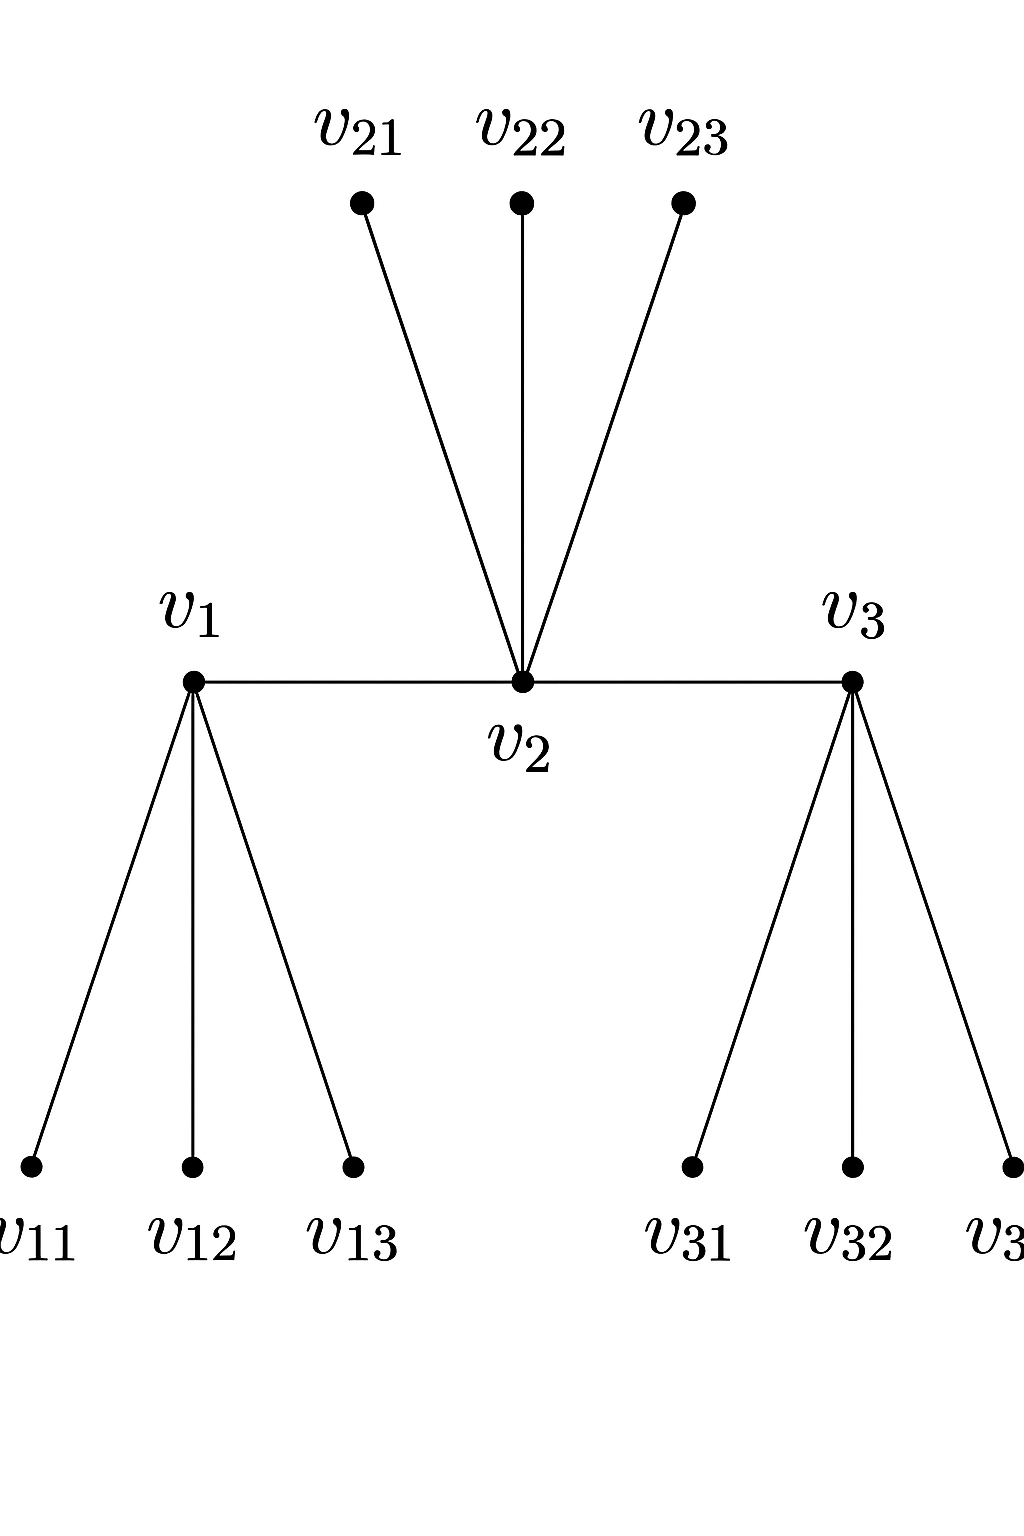
\includegraphics[width=0.4\linewidth]{graf 1.png}
        \end{figure}
        
        Buatlah matriks \textit{adjacency} berdasarkan struktur graf $G$ tersebut.
        
        \item (Nilai max: 5) Berdasarkan graf $G$ pada poin (b), graf apa yang dihasilkan jika graf $G$ dikenakan operasi \textit{join} (+) dengan graf lengkap $K_1$.
        
        \item (Nilai max: 5) Selidiki apakah graf roda (\textit{wheel}) $W_n$ dapat dikatakan sebagai hasil operasi \textit{join} graf \textit{cycle} $C_n$ dengan graf lengkap $K_1$.
    \end{enumerate}

    \item (Nilai max: 20) Diberikan graf sebagai berikut.

    \begin{figure}[H]
        \centering
        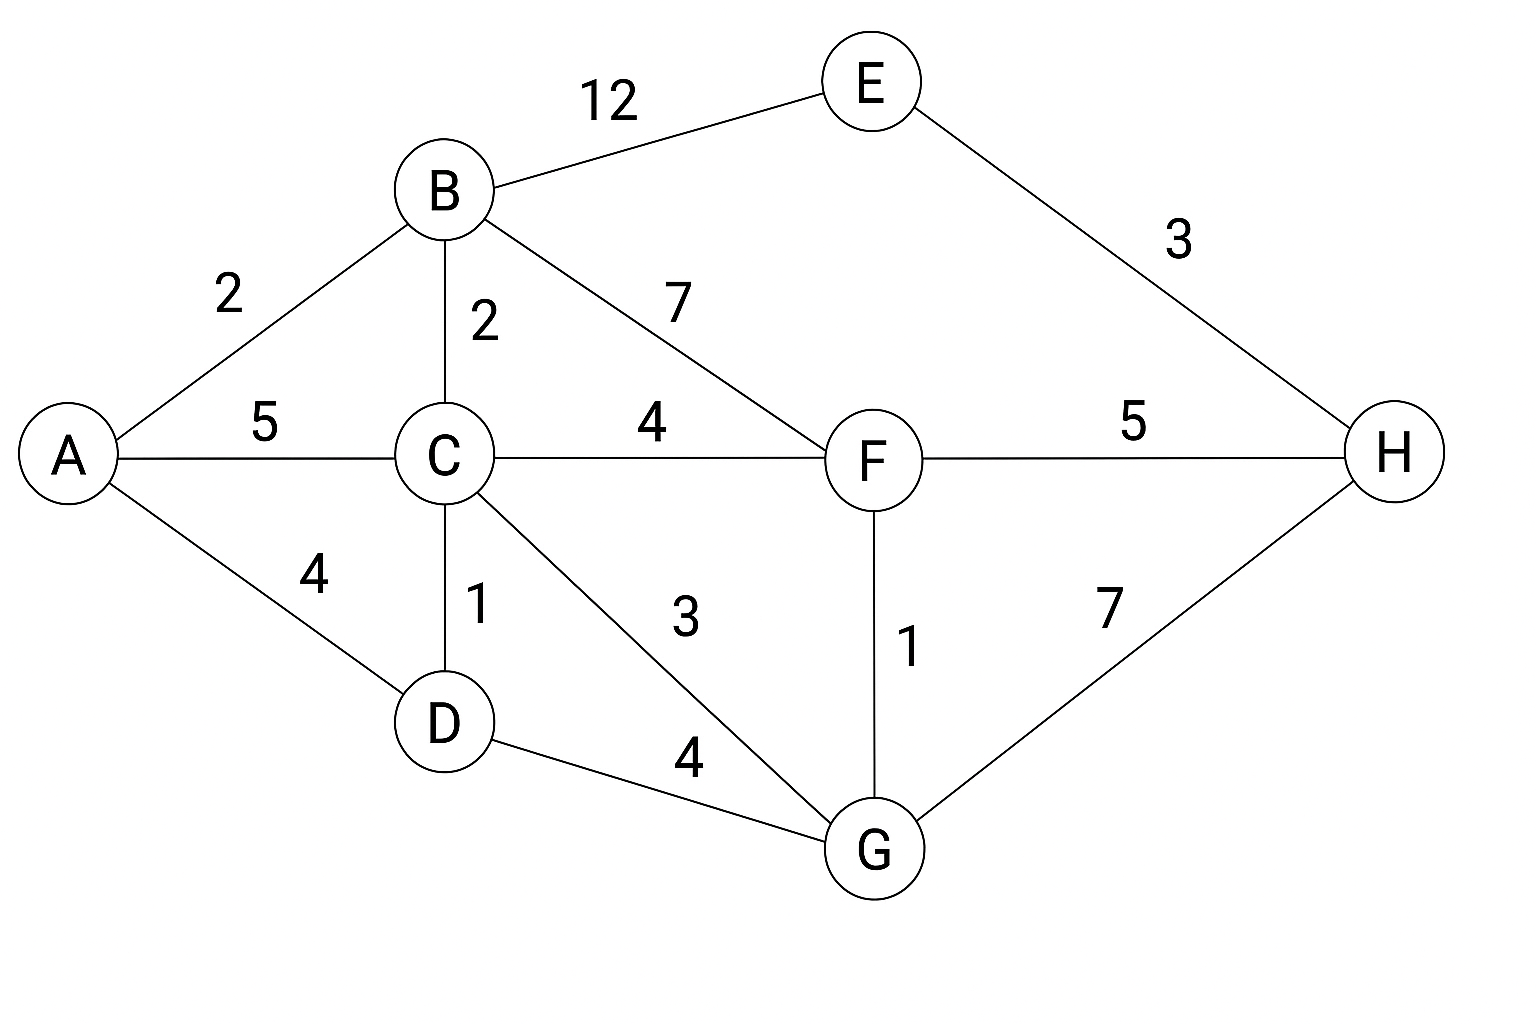
\includegraphics[width=0.6\linewidth]{graf 2.png}
    \end{figure}
    
    Dengan menggunakan algoritma Dijkstra, cari lintasan terpendek dari $A$ ke $H$.

    \item (Nilai max: 20) Diketahui Frekuensi dari Alfabet sebagai berikut.
    
    \begin{center}
        \begin{tabular}{|c|c||c|c|}
            \hline
            Letter & Frequency & Letter & Frequency \\
            \hline
            A & 77 & N & 67 \\
            B & 17 & O & 67 \\
            C & 32 & P & 20 \\
            D & 42 & Q & 5 \\
            E & 120 & R & 59 \\
            F & 24 & S & 67 \\
            G & 17 & T & 85 \\
            H & 50 & U & 37 \\
            I & 76 & V & 12 \\
            J & 4 & W & 22 \\
            K & 7 & X & 4 \\
            L & 42 & Y & 22 \\
            M & 24 & Z & 2 \\
            \hline
        \end{tabular}
    \end{center}
    
    Gambar 1: Tabel frekuensi dari tiap alfabet
    
    Dapatkan Kode Huffman untuk setiap huruf pada \textit{string} AKU CINTA ITS.

    \item (Nilai max: 20) Diketahui \textit{PreOrder traversal} dari suatu \textit{binary tree} adalah A B D G M H C E J N F K O L, sedangkan \textit{InOrder traversal}-nya adalah G M D H B A N J E C K O F L. Gambarkan \textit{binary tree} yang dimaksud!

    \item Diberikan \textit{phrase-structure grammar} $G = (V, T, S, P)$ dengan \textit{vocabulary} $V = \{S, A, B, a, b\}$, simbol \textit{terminal} $T = \{a, b\}$, dan produksi $P$ yang terdiri dari $S \rightarrow Sa, S \rightarrow AB, A \rightarrow aA, A \rightarrow a, B \rightarrow ba$.
    
    \begin{enumerate}
        \item (Nilai max: 8) Carilah $L(G)$, yaitu himpunan \textit{language} yang dibangkitkan oleh \textit{grammar} $G$.
        
        \item (Nilai max: 12) Selidiki apakah $G$ merupakan \textit{grammar} tipe 0, tipe 1, tipe 2, atau tipe 3. Jelaskan jawaban Anda.
    \end{enumerate}

    \item Diberikan \textit{finite-state machine} $M = (S, I, O, f, g, s_0)$ dengan himpunan \textit{state} $S$, himpunan simbol \textit{input} $I$, himpunan simbol \textit{output} $O$, fungsi transisi $f$ yang memetakan setiap \textit{state} dengan \textit{input} ke \textit{state} baru, fungsi transisi $g$ yang memetakan setiap \textit{state} dengan \textit{input} ke \textit{output}, \textit{starting state} $s_0$, yang dinyatakan dalam tabel transisi berikut.
    
    \begin{center}
        \begin{tabular}{|c|c|c|c|c|}
            \hline
            & \multicolumn{2}{c|}{f} & \multicolumn{2}{c|}{g} \\
            \hline
            State & \multicolumn{2}{c|}{Input} & \multicolumn{2}{c|}{Input} \\
            \hline
            & 0 & 1 & 0 & 1 \\
            \hline
            $s_0$ & $s_0$ & $s_4$ & 1 & 1 \\
            $s_1$ & $s_0$ & $s_3$ & 0 & 1 \\
            $s_2$ & $s_0$ & $s_2$ & 0 & 0 \\
            $s_3$ & $s_1$ & $s_2$ & 1 & 1 \\
            $s_4$ & $s_1$ & $s_0$ & 1 & 0 \\
            \hline
        \end{tabular}
    \end{center}
    
    \begin{enumerate}
        \item (Nilai max: 8) Gambarkan diagram \textit{state} dari \textit{finite-state machine} $M$.
        
        \item (Nilai max: 6) Carilah \textit{output} dari mesin diatas jika diberikan \textit{input} 101011011. Jelaskan jawaban Anda.
        
        \item (Nilai max: 6) Berdasarkan \textit{output} yang diperoleh pada bagian (b), selidiki apakah \textit{output} tersebut termuat pada \textit{concatenation} antara $A$ dan $B^*$, yaitu $AB^*$, dengan $A = \{111\}$ dan $B = \{0, 1\}$.
    \end{enumerate}

    \item Diberikan mesin \textit{Nondeterministic Finite Automata} (NFA) $M = (S, I, f, s_0, F)$ dengan himpunan \textit{state} $S$, himpunan simbol \textit{input} $I$, fungsi transisi $f$ yang memetakan setiap \textit{state} dengan \textit{input} ke \textit{state} berikutnya, \textit{starting state} $s_0$, dan himpunan \textit{state} akhir (\textit{final}) $F$ dengan $F = \{s_0, s_1, s_2, s_4\} \subseteq S$, yang digambarkan oleh diagram otomata berikut.
    

    Berdasarkan diagram otomata tersebut, jawablah pertanyaan ini.
    
    \begin{enumerate}
        \item (Nilai max: 6) Carilah $L(M)$. Jelaskan jawaban Anda.
        
        \item (Nilai max: 6) Buatlah tabel transisi dari mesin $M$.
        
        \item (Nilai max: 8) Ubahlah NFA diatas menjadi \textit{Deterministic Finite Automata} (DFA) dan gambarkan diagram otomatanya.
    \end{enumerate}
\end{enumerate}

\centering{\large \textbf{SELAMAT MENGERJAKAN}}

\end{document}